% !TEX root = ../diff_equations.tex
% =================================================================
%  sections/lecture01.tex
%  Лекция 1. Основные понятия. Задача Коши. Интеграл уравнения.
%
%  Места под иллюстрации отмечены комментарием «РИСУНОК N»:
%  внутри каждой заготовки tikzpicture нарисованы только оси,
%  содержательная часть дорисовывается позже.
% =================================================================

\part*{Лекция 1}

\section{Основные понятия. Задача Коши. Интеграл уравнения}

Всюду далее независимая переменная --- $x$ (позже $t$), искомая функция ---
$y(x)$ (позже $x(t)$).

\subsection{Дифференциальное уравнение и его решение}

\begin{Definition}{Дифференциальное уравнение}{ду}
	\textbf{Дифференциальное уравнение} --- уравнение вида
	\[
	F\bigl(x,\,y,\,y',\,\dots,\,y^{(n)}\bigr) = 0,
	\]
	где $n$ --- \textbf{порядок} дифференциального уравнения.
\end{Definition}

\begin{Example}{Второй закон Ньютона}{}
	Ускорение тела прямо пропорционально равнодействующей всех сил, приложенных к нему, и обратно пропорционально его массе.
	Если равнодействующая всех сил выражается через время, положение тела и его скорость, то
	\[
	m\ddot{x} = f(t,\,x,\,\dot{x})
	\]
	--- дифференциальное уравнение второго порядка.
\end{Example}

Далее рассматривается дифференциальное уравнение первого порядка,
\textbf{разрешённое относительно производной}:
\[
y' = f(x,y), \qquad y' = \dder{y}{x}
\]
$x$ --- независимая переменная, $y$ --- искомая функция.

\begin{Remark}{Соглашения курса}{}
	Всюду далее $f$ непрерывна: $G \subset \RR^2$ --- область
	(открытое множество), $f \in C(G)$.
\end{Remark}

\begin{Definition}{}{решение}
	Функция $y : (a,b) \to \RR$ называется \textbf{решением} на $(a,b)$, если
	\begin{enumerate}
		\item $\exists\, y'(x)$ на $(a,b)$;
		\item $(x, y(x)) \in G$ $\ \forall x \in (a,b)$;
		\item $y'(x) = f\bigl(x, y(x)\bigr)$ на $(a,b)$.
	\end{enumerate}
	График решения называется \textbf{интегральной кривой}.
\end{Definition}

\begin{Example}{}{экспонента}
	$y' = ky$, $k > 0$, $G = \RR^2$. Тогда
	\[
	\forall C \in \RR \colon \quad y(x) = C e^{kx}
	\]
	--- решение на любом интервале $(a,b)$.
\end{Example}

% ---------------------------------------------------------------
% ---------------------------------------------------------------
% РИСУНОК 1: семейство интегральных кривых y = C e^{kx} (k = 1).
% Шаг по C неравномерный (0.12, 0.3, 0.65, 1.3) — так кривые
% ложатся на лист равномернее, чем при постоянном шаге.
% ---------------------------------------------------------------
\begin{figure}[H]
	\centering
	\begin{tikzpicture}[x=1.35cm, y=1.0cm, >=Stealth]
		\draw[ax] (-2.5,0) -- (2.95,0) node[right] {$x$};
		\draw[ax] (0,-2.45) -- (0,2.75) node[above] {$y$};
		\foreach \x in {-1,1,2} \draw[tickmark] (\x,0.07) -- (\x,-0.07);
		
		\begin{scope}
			\clip (-2.1,-2.35) rectangle (2.65,2.4);
			\foreach \c in {0.12, 0.3, 0.65, 1.3}{
				\draw[curve, domain=-2.1:2.65, samples=120] plot (\x,{\c*exp(\x)});
				\draw[curve, domain=-2.1:2.65, samples=120] plot (\x,{-\c*exp(\x)});
			}
		\end{scope}
		
		% C = 0 — стационарное решение, совпадает с осью Ox
		\draw[curve, very thick] (-2.1,0) -- (2.65,0);
		\node[slbl, below] at (1.9,-0.08) {$C = 0$};
		
		\node[lbl] at (-1.6,1.15) {$C > 0$};
		\node[lbl] at (-1.6,-1.15) {$C < 0$};
	\end{tikzpicture}
	\caption{Семейство интегральных кривых $y = Ce^{kx}$ уравнения $y' = ky$
		при $k > 0$.}
	\label{fig:семейство-экспонент}
\end{figure}

\begin{Remark}{Другие постановки}{}
	Помимо поиска всех решений встречаются задачи об ограниченных
	решениях, о периодических решениях и т.\,д.
\end{Remark}

\subsection{Задача Коши}

\begin{Definition}{Решение задачи Коши}{коши}
	Пусть фиксирована точка $(x_0, y_0) \in G$. Функция $y(x)$ ---
	\textbf{решение задачи Коши} с начальными данными $(x_0,y_0)$, если
	\begin{enumerate}
		\item $y(x)$ --- решение на некотором $(a,b) \ni x_0$;
		\item $y(x_0) = y_0$.
	\end{enumerate}
\end{Definition}

\begin{Example}{}{}
	Для $y' = ky$ и точки $(x_0,y_0)$ решением задачи Коши будет
	\[
	y(x) = y_0\, e^{k(x - x_0)}.
	\]
\end{Example}

% ---------------------------------------------------------------
% РИСУНОК 2: начальное условие выделяет одну кривую семейства.
% Серым — семейство y = Ce^{kx}, фиолетовым — решение через (x_0,y_0).
% ---------------------------------------------------------------
\begin{figure}[H]
	\centering
	\begin{tikzpicture}[x=1.35cm, y=1.0cm, >=Stealth]
		\draw[ax] (-2.5,0) -- (2.95,0) node[right] {$x$};
		\draw[ax] (0,-2.45) -- (0,2.75) node[above] {$y$};
		
		\begin{scope}
			\clip (-2.1,-2.35) rectangle (2.65,2.4);
			% семейство: те же значения C, что и на рис. 1.1
			\foreach \c in {0.12, 0.3, 0.65, 1.3}{
				\draw[curve, domain=-2.1:2.65, samples=120] plot (\x,{\c*exp(\x)});
				\draw[curve, domain=-2.1:2.65, samples=120] plot (\x,{-\c*exp(\x)});
			}
			\draw[curve, very thick] (-2.1,0) -- (2.65,0);
			% решение задачи Коши: C = y_0 e^{-x_0} при x_0 = 0.6, y_0 = 1
			\draw[curvehl, domain=-2.1:2.65, samples=120] plot (\x,{exp(\x-0.6)});
		\end{scope}
		
		\draw[curveaux] (0.6,0) -- (0.6,1) -- (0,1);
		\node[pt, Purple] at (0.6,1) {};
		\node[slbl, below] at (0.6,-0.06) {$x_0$};
		\node[slbl, left]  at (-0.06,1) {$y_0$};
		
		\node[Purple, lbl] at (-1.15,2.15) {$y = y_0 e^{k(x-x_0)}$};
		\draw[-{Stealth[length=2mm]}, Purple] (0.15,2.1) -- (1.1,1.85);
	\end{tikzpicture}
	\caption{Начальное условие $y(x_0) = y_0$ выделяет из семейства
		$y = Ce^{kx}$ (серое) ровно одну интегральную кривую (фиолетовая):
		константа определяется однозначно, $C = y_0 e^{-kx_0}$, и решение
		задачи Коши имеет вид $y(x) = y_0 e^{k(x-x_0)}$.}
	\label{fig:задача-коши}
\end{figure}

\subsection{Единственность}

\begin{Definition}{Точка единственности}{точка-единственности}
	Точка $(x_0,y_0) \in G$ --- \textbf{точка единственности}, если для любых
	решений $y_1(x)$, $y_2(x)$ задачи Коши с начальными данными $(x_0,y_0)$
	\[
	\exists\, (\alpha,\beta) \ni x_0 \colon \quad
	y_1(x) \equiv y_2(x), \quad x \in (\alpha,\beta).
	\]
\end{Definition}

\begin{Example}{Нарушение единственности}{нарушение-единственности}
	$y' = 3\sqrt[3]{y^{2}}$, $f \in C(\RR^2)$, начальная точка $(0,0)$.
	
	\medskip
	Первое решение:
	\[
	y_1(x) =
	\begin{cases}
		0,   & x \le 0,\\
		x^3, & x \ge 0.
	\end{cases}
	\]
	При $x \ge 0$ действительно $y_1' = 3x^2 = 3\sqrt[3]{x^{6}}$.
	
	\medskip
	Второе решение: $y_2(x) \equiv 0$, $x \in \RR$.
	
	\medskip
	Значит, $(0,0)$ --- \textbf{не точка единственности}.
\end{Example}

% ---------------------------------------------------------------
% РИСУНОК 3: два (и более) решения через точку (0,0):
% нулевое решение и кривая, отрывающаяся от нуля в разные моменты
% ---------------------------------------------------------------
\begin{figure}[H]
	\centering
	\begin{tikzpicture}[x=1.25cm, y=0.85cm, >=Stealth]
		\draw[ax] (-2.7,0) -- (2.95,0) node[right] {$x$};
		\draw[ax] (0,-2.5) -- (0,2.7) node[above] {$y$};
		
		\begin{scope}
			\clip (-2.55,-2.4) rectangle (2.75,2.45);
			% y_1: 0 при x <= 0 и x^3 при x >= 0
			\draw[curvehl, domain=0:1.4, samples=80] plot (\x,{\x*\x*\x});
			\draw[curve, domain=0.3:1.7, samples=80] plot (\x,{(\x - 0.3)*(\x - 0.3)*(\x - 0.3)});
			\draw[curve, domain=0.6:2.0, samples=80] plot (\x,{(\x - 0.6)*(\x - 0.6)*(\x - 0.6)});
			\draw[curve, domain=0.9:2.3, samples=80] plot (\x,{(\x - 0.9)*(\x - 0.9)*(\x - 0.9)});
			\draw[curve, domain=-2.3:-0.9, samples=80] plot (\x,{(\x + 0.9)*(\x + 0.9)*(\x + 0.9)});
			\draw[curve, domain=-2.0:-0.6, samples=80] plot (\x,{(\x + 0.6)*(\x + 0.6)*(\x + 0.6)});
			\draw[curve, domain=-1.7:-0.3, samples=80] plot (\x,{(\x + 0.3)*(\x + 0.3)*(\x + 0.3)});
			\draw[curve, domain=-1.4:0, samples=80] plot (\x,{\x*\x*\x});
		\end{scope}

		% нулевое решение — совпадает с осью Ox
		\draw[curvehl] (-2.1,0) -- (2.65,0);
		
		\node[pt] at (0,0) {};
		\node[slbl, below left] at (0,-0.05) {$0$};
		\node[Purple, lbl, left] at (1.05,2.0) {$y_1$};
		\node[Purple, slbl, above] at (-2.0,0.1) {$y_2 \equiv 0$};
	\end{tikzpicture}
	\caption{Через точку $(0,0)$ проходит бесконечно много решений уравнения
		$y' = 3\sqrt[3]{y^{2}}$, в том числе решение $y_2 \equiv 0$ и решение
		$y_1$ (равное $x^3$ при $x \ge 0$). Поскольку $\forall \varepsilon > 0: x^3 > 0$, $y_1$ и $y_2$ не совпадают ни в какой окрестности точки $0$}
	\label{fig:неединственность}
\end{figure}

% TODO (сверить с лектором): проговаривалось ли, что причина
% неединственности — разрыв \pder{f}{y} в точке (0,0)?

\subsection{Две основные теоремы (без доказательства)}

\begin{Theorem}{Существование}{существование}
	Пусть $y' = f(x,y)$, $f \in C(G)$. Тогда
	\[
	\forall (x_0,y_0) \in G \quad \exists\ \text{решение задачи Коши}
	\]
	с начальными данными $(x_0,y_0)$.
\end{Theorem}

\begin{Theorem}{Единственность}{единственность}
	Пусть $y' = f(x,y)$, причём $f,\ \pder{f}{y} \in C(G)$. Тогда всякая точка
	$(x_0,y_0) \in G$ --- точка единственности.
\end{Theorem}

\subsection{Поле направлений}

Пусть $y' = f(x,y)$, $y(x)$ --- решение на $(a,b)$, $x_0 \in (a,b)$,
$y_0 = y(x_0)$. Тогда
\[
y'(x_0) = f\bigl(x_0, y(x_0)\bigr) = f(x_0,y_0),
\]
то есть $y'(x_0)$ --- угловой коэффициент касательной к интегральной кривой
в точке $x_0$: $k = f(x_0,y_0)$.

% ---------------------------------------------------------------
% РИСУНОК 4: интегральная кривая и касательная в точке (x_0, y_0)
% с угловым коэффициентом k = f(x_0, y_0)
% ---------------------------------------------------------------
\begin{figure}[H]
	\centering
	\begin{tikzpicture}[x=1.3cm, y=1.3cm, >=Stealth]
		\draw[ax] (-0.4,0) -- (4.0,0) node[below right] {$x$};
		\draw[ax] (0,-0.4) -- (0,3.15) node[above] {$y$};
		
		% интегральная кривая y(x) = 0.18x^2 + 0.25x + 0.35
		\draw[curvehl, domain=0.1:3.1, samples=120]
		plot (\x,{0.18*\x*\x + 0.25*\x + 0.35});
		\node[Purple, slbl, above left] at (3.1,2.85) {$y(x)$};
		
		% касательная в точке x_0 = 1.8: k = 0.36*1.8 + 0.25 = 0.898
		\draw[curve, thick] (0.6,0.3032) -- (3.15,2.5936);
		\node[Blue, slbl, right] at (3.18,2.55) {касательная};
		
		% точка касания и проекции на оси
		\draw[curveaux] (1.8,0) -- (1.8,1.3832) -- (0,1.3832);
		\node[pt] at (1.8,1.3832) {};
		\node[slbl, below] at (1.8,-0.06) {$x_0$};
		\node[slbl, left]  at (-0.06,1.3832) {$y_0$};
		
		% треугольник наклона: сдвиг на 1 вправо даёт подъём k
		\draw[curveaux] (1.8,1.3832) -- (2.8,1.3832) -- (2.8,2.2812);
		\node[slbl, below] at (2.3,1.36) {$1$};
		\node[slbl, right] at (2.83,1.83) {$k = f(x_0,y_0)$};
	\end{tikzpicture}
	\caption{Угловой коэффициент касательной к интегральной кривой в точке
		$(x_0,y_0)$ равен $f(x_0,y_0)$: он определяется самим уравнением и не
		зависит от того, какое решение через эту точку проходит. Поэтому в
		каждой точке области $G$ направление интегральной кривой известно
		заранее.}
	\label{fig:касательная}
\end{figure}

\begin{Definition}{Поле направлений (не было на лекции)}{поле-направлений}
	\textbf{Полем направлений} уравнения $y' = f(x,y)$ называется соответствие,
	сопоставляющее каждой точке $(x,y) \in G$ прямую $\ell(x,y)$, проходящую
	через эту точку с угловым коэффициентом $f(x,y)$:
	\[
	\ell(x,y) = \bigl\{(\xi,\eta) \in \RR^2 \colon
	\eta - y = f(x,y)\,(\xi - x)\bigr\}.
	\]
	Изображают его, рисуя в точках $(x,y)$ короткие штрихи с наклоном $f(x,y)$.
	
	\medskip
	Говорят, что кривая \textbf{касается поля направлений} в точке $(x_0,y_0)$,
	если она имеет в этой точке касательную и эта касательная совпадает
	с $\ell(x_0,y_0)$.
\end{Definition}

Поле направлений строится для всех $(x,y) \in G$.

\begin{Statement}{}{касание}
	Интегральная кривая касается поля направлений в каждой своей точке.
\end{Statement}

\begin{Definition}{Изоклина}{изоклина}
	\textbf{Изоклиной} числа $k$ называется множество
	\[
	\{(x,y) \in G \colon f(x,y) = k\}.
	\]
\end{Definition}

% ---------------------------------------------------------------
% РИСУНОК 5: поле направлений (сетка штрихов) и несколько изоклин
% f(x,y) = k для разных k
% ---------------------------------------------------------------
\begin{figure}[H]
	\centering
	\begin{tikzpicture}[x=1.42cm, y=1.42cm, >=Stealth]
		% поле направлений уравнения y' = x - y:
		% в каждом узле сетки — штрих с наклоном k = x - y
		\foreach \i in {-2.25,-1.95,...,2.26}{
			\foreach \j in {-2.25,-1.95,...,2.26}{
				\pgfmathsetmacro{\ang}{atan(\i-\j)}
				\draw[black!45, line width=0.35pt, shift={(\i,\j)}, rotate=\ang]
				(-0.11,0) -- (0.11,0);
			}
		}
		
		\draw[ax] (-2.6,0) -- (2.75,0) node[below right] {$x$};
		\draw[ax] (0,-2.6) -- (0,2.75) node[above] {$y$};
		
		\begin{scope}
			\clip (-2.45,-2.45) rectangle (2.45,2.45);
			% изоклины: x - y = k, то есть прямые y = x - k
			\draw[curveaux] (-2.45,-2.45) -- (2.45,2.45);
			\draw[curveaux] (-0.45,-2.45) -- (2.45,0.45);
			% решения y = x - 1 + C e^{-x}
			\foreach \c in {0.35, 1.2, -0.6}{
				\draw[curve, domain=-2.45:2.45, samples=200]
				plot (\x,{\x-1+\c*exp(-\x)});
			}
			% C = 0: изоклина k = 1 сама является решением
			\draw[curvehl] (-2.45,-3.45) -- (2.45,1.45);
		\end{scope}
		
		% подписи вынесены за поле, к правым концам прямых
		\node[slbl, black!60, right] at (2.5,2.45) {$k = 0$};
		\node[Purple, slbl, right]   at (2.5,1.45) {$k = 1$};
		\node[slbl, black!60, right] at (2.5,0.45) {$k = 2$};
	\end{tikzpicture}
	\caption{Поле направлений уравнения $y' = x - y$: в каждой точке отложен
		короткий штрих с угловым коэффициентом $k = f(x,y)$. Изоклины здесь ---
		прямые $y = x - k$ (пунктир), вдоль каждой из них все штрихи
		параллельны. Синие кривые $y = x - 1 + Ce^{-x}$ --- решения: в каждой
		своей точке они касаются поля. Изоклина $k = 1$, то есть прямая
		$y = x - 1$ (фиолетовая), сама оказывается решением, и остальные
		интегральные кривые приближаются к ней при $x \to +\infty$.}
	\label{fig:поле-направлений}
\end{figure}

\subsection{Интегрируемые типы уравнений первого порядка}

\textbf{Тип 1:} $y' = f(x)$, $f \in C(a,b)$

Из математического анализа: для любых $(x_0,y_0)$, где $x_0 \in (a,b)$,
\[
y(x) = y_0 + \int_{x_0}^{x} f(t)\,\dd t, \qquad x_0,\, x \in (a,b).
\]

\textbf{Тип 2:} уравнения с разделяющимися переменными (дальше)

Есть еще типы, но мы пока говорим об этих двух.

\subsection{Интеграл уравнения}

Пусть $y' = f(x,y)$, $f \in C(G)$, $H \subset G$ --- область.

\begin{Definition}{Интеграл}{интеграл}
	Функция $u(x,y)$ --- \textbf{интеграл} в $H$, если
	\begin{enumerate}
		\item $u \in C^1(H,\RR)$;
		\item $\pder{u}{y} \neq 0$ в $H$;
		\item если $y(x)$, $x \in (a,b)$, --- решение и
		$(x,y(x)) \in H\ \ \forall x \in (a,b)$, то
		$u\bigl(x, y(x)\bigr) = \const$ на $(a,b)$.
	\end{enumerate}
\end{Definition}

\begin{Example}{Интеграл уравнения $y' = ky$}{интеграл-экспонента}
	Пусть $y' = ky$, $G = \RR^2$ (пример из п.~1.1). Положим
	\[
	u(x,y) = y\,e^{-kx}, \qquad H = G = \RR^2 .
	\]
	Проверим три пункта определения.
	\begin{enumerate}
		\item $u \in C^1(\RR^2,\RR)$ как произведение гладких функций.
		\item $\pder{u}{y}(x,y) = e^{-kx} \neq 0$ всюду в $\RR^2$.
		\item Пусть $y(x)$ --- произвольное решение на $(a,b)$. Тогда
		\[
		\dder{}{x}\Bigl[y(x)\,e^{-kx}\Bigr]
		= y'(x)\,e^{-kx} - k\,y(x)\,e^{-kx}
		= \bigl(y'(x) - k\,y(x)\bigr)e^{-kx} = 0,
		\]
		так как $y' = ky$. Значит $u\bigl(x,y(x)\bigr) = \const$ на $(a,b)$.
	\end{enumerate}
	Таким образом, $u$ --- интеграл в $\RR^2$, а общий интеграл имеет вид
	$y\,e^{-kx} = C$. Разрешая его относительно $y$, получаем уже известное
	семейство $y = C e^{kx}$.
\end{Example}

% ---------------------------------------------------------------
% РИСУНОК 7: поверхность z = u(x,y) = y e^{-kx}, её линии уровня
% и их проекции на Oxy — интегральные кривые y = C e^{kx}.
% Аксонометрия задана векторами x/y/z в опциях tikzpicture.
% ---------------------------------------------------------------
\begin{figure}[H]
	\centering
	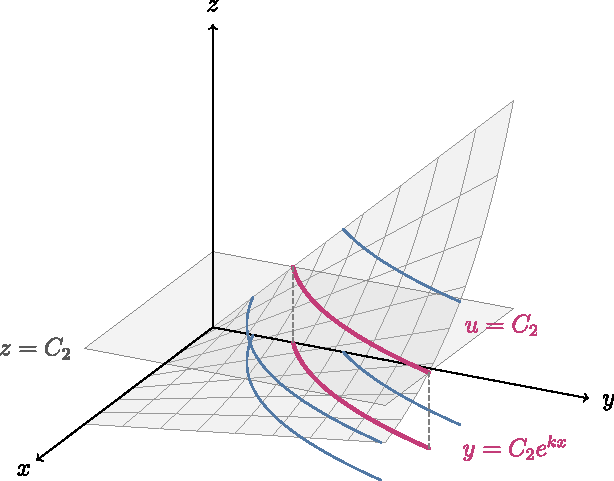
\includegraphics{figures/fig07-integral-surface.pdf}
	\caption{Интеграл $u(x,y) = y e^{-kx}$ уравнения $y' = ky$ как поверхность
		$z = u(x,y)$. Сечение поверхности горизонтальной плоскостью $z = C$ даёт
		линию уровня интеграла; её проекция на плоскость $Oxy$ (внизу) --- в
		точности интегральная кривая $y = C e^{kx}$. Пункт~3 определения интеграла
		означает, что вдоль каждой такой кривой «высота» $u$ не меняется, а
		константа $C$ служит номером кривой в семействе.}
	\label{fig:интеграл-поверхность}
\end{figure}

\begin{Remark}{Линии уровня интеграла}{линии-уровня}
	Рисунок~\ref{fig:интеграл-поверхность} даёт удобный способ читать
	определение интеграла. Интеграл $u$ --- это функция двух переменных, то есть
	поверхность $z = u(x,y)$ над областью $H$. Её \textbf{линией уровня} называется
	множество
	\[
	L_C = \{(x,y) \in H \colon u(x,y) = C\},
	\]
	то есть проекция на плоскость $Oxy$ сечения поверхности горизонтальной
	плоскостью $z = C$.

	В этих терминах пункт~3 определения интеграла читается так: график каждого решения
	целиком лежит в одной линии уровня.

	Отсюда видно, почему функция от интеграла (утверждение~1.2) --- снова
	интеграл: строго монотонная $g$ меняет высоту поверхности, но не сами сечения,
	поэтому линии уровня $g(u)$ совпадают с линиями уровня $u$.
\end{Remark}

% --- прежний вариант рисунка 7 (TikZ-аксонометрия), оставлен на всякий случай ---
% \begin{figure}[H]
% 	\centering
% 	\begin{tikzpicture}[
% 		x={(0.95cm,-0.42cm)}, y={(1.05cm,0.30cm)}, z={(0cm,1.05cm)},
% 		>=Stealth]
%
% 		% горизонтальная плоскость z = C_2
% 		\fill[black!10, opacity=0.45]
% 		(0,0,0.8) -- (2,0,0.8) -- (2,3,0.8) -- (0,3,0.8) -- cycle;
%
% 		\draw[ax] (0,0,0) -- (2.6,0,0) node[below] {$x$};
% 		\draw[ax] (0,0,0) -- (0,3.6,0) node[right] {$y$};
% 		\draw[ax] (0,0,0) -- (0,0,3.4) node[above] {$z$};
%
% 		% каркас поверхности z = y e^{-x}
% 		\foreach \yy in {1,2,3}{
% 			\draw[curveaux, black!35, domain=0:2, samples=60]
% 			plot (\x, \yy, {\yy*exp(-\x)});
% 		}
% 		\foreach \xx in {0,0.5,1,1.5,2}{
% 			\draw[curveaux, black!35] (\xx,0,0) -- (\xx,3,{3*exp(-\xx)});
% 		}
% 		% границы поверхности
% 		\draw[black!55, thin, domain=0:2, samples=60] plot (\x,3,{3*exp(-\x)});
% 		\draw[black!55, thin] (0,0,0) -- (0,3,3);
% 		\draw[black!55, thin] (2,0,0) -- (2,3,{3*exp(-2)});
%
% 		% линии уровня u = C на поверхности и их проекции на Oxy
% 		\draw[curve, domain=0:2.00, samples=60] plot (\x,{0.4*exp(\x)},0.4);
% 		\draw[curve, domain=0:2.00, samples=60] plot (\x,{0.4*exp(\x)},0);
% 		\draw[curve, domain=0:0.83, samples=60] plot (\x,{1.3*exp(\x)},1.3);
% 		\draw[curve, domain=0:0.83, samples=60] plot (\x,{1.3*exp(\x)},0);
%
% 		\draw[curvehl, domain=0:1.32, samples=60] plot (\x,{0.8*exp(\x)},0.8);
% 		\draw[curvehl, domain=0:1.32, samples=60] plot (\x,{0.8*exp(\x)},0);
% 		\draw[curveaux, black!55] (0,0.8,0.8) -- (0,0.8,0);
% 		\draw[curveaux, black!55] (1.32,2.99,0.8) -- (1.32,2.99,0);
%
% 		\node[slbl, black!60] at (2.35,0,0.8) {$z = C_2$};
% 		\node[Purple, slbl] at (1.55,3.35,0.8) {$u = C_2$};
% 		\node[Purple, slbl] at (1.60,3.40,0) {$y = C_2 e^{kx}$};
% 	\end{tikzpicture}
% 	\caption{Интеграл $u(x,y) = y e^{-kx}$ уравнения $y' = ky$ как поверхность
% 		$z = u(x,y)$. Сечение поверхности горизонтальной плоскостью $z = C$ даёт
% 		линию уровня интеграла; её проекция на плоскость $Oxy$ (внизу) --- в
% 		точности интегральная кривая $y = C e^{kx}$. Пункт~3 определения интеграла
% 		означает, что вдоль каждой такой кривой «высота» $u$ не меняется, а
% 		константа $C$ служит номером кривой в семействе.}
% 	\label{fig:интеграл-поверхность}
% \end{figure}

\begin{Statement}{Функция от интеграла}{функция-от-интеграла}
	Если $u$ --- интеграл в $H$, то для любой $g \in C^1$ с $g' \neq 0$
	функция $v = g(u)$ --- тоже интеграл в $H$.
\end{Statement}

\begin{proof}
	Пусть $u$ --- интеграл в $H$, а $g \in C^1(\Delta)$, $g' \neq 0$ на $\Delta$,
	где $\Delta$ --- промежуток, содержащий $u(H)$. Проверим для $v = g \circ u$
	все три пункта определения интеграла.

	\medskip
	\textbf{Шаг 1 (гладкость).} Так как $u \in C^1(H)$ и $g \in C^1(\Delta)$,
	\[
	\pder{v}{x}(x,y) = g'\bigl(u(x,y)\bigr)\cdot \pder{u}{x}(x,y),
	\qquad
	\pder{v}{y}(x,y) = g'\bigl(u(x,y)\bigr)\cdot \pder{u}{y}(x,y).
	\]
	Функция $g' \circ u$ непрерывна в $H$ как композиция непрерывных, а
	$\pder{u}{x}, \pder{u}{y} \in C(H)$. Значит, обе частные производные $v$
	непрерывны в $H$, то есть $v \in C^1(H,\RR)$.

	\medskip
	\textbf{Шаг 2 (невырожденность).}
	\[
	\pder{v}{y} = g'(u)\cdot\pder{u}{y} \neq 0 \quad \text{в } H.
	\]
	Оба множителя не равны 0 во всех $(x,y) \in H$: $g'(u)  \neq 0$ по условию на $g$, $\pder{u}{y} \neq 0$ по определеню интеграла.

	\medskip
	\textbf{Шаг 3 (постоянство вдоль решений).} Пусть $y(x)$, $x \in (a,b)$, ---
	решение уравнения и $(x,y(x)) \in H$ при всех $x \in (a,b)$. По пункту 3
	определения для $u$ найдётся $C_0$ с $u\bigl(x,y(x)\bigr) \equiv C_0$ на
	$(a,b)$. Тогда
	\[
	v\bigl(x,y(x)\bigr) = g\Bigl(u\bigl(x,y(x)\bigr)\Bigr) = g(C_0) = \const
	\quad \text{на } (a,b).
	\]

	Все три пункта выполнены, значит $v = g(u)$ --- интеграл в $H$.
\end{proof}

\begin{Statement}{Необходимое и достаточное условие интеграла}{нид-интеграл}
	Функция $u$ является интегралом тогда и только тогда, когда
	\[
	\pder{u}{x}(x,y) + \pder{u}{y}(x,y)\, f(x,y) \equiv 0 .
	\]
\end{Statement}

\begin{proof}
	Всюду считаем выполненными пункты 1--2 определения интеграла:
	$u \in C^1(H,\RR)$ и $\pder{u}{y} \neq 0$ в $H$; доказывается
	равносильность пункта 3 указанному тождеству.

	\medskip
	\textbf{Шаг 1 (необходимость).} Пусть $u$ --- интеграл в $H$. Зафиксируем
	произвольную точку $(x_0,y_0) \in H$. Так как $f \in C(G)$, по теореме
	существования найдётся решение $y(x)$ задачи Коши с начальными данными
	$(x_0,y_0)$, определённое на некотором интервале $(a,b) \ni x_0$.

	Функция $y$ непрерывна, $y(x_0) = y_0$, а $H$ открыто, поэтому найдётся
	$(\alpha,\beta) \subset (a,b)$, $x_0 \in (\alpha,\beta)$, для которого
	$\bigl(x,y(x)\bigr) \in H$ при всех $x \in (\alpha,\beta)$; сузим решение
	на этот интервал.

	По пункту 3 определения $u\bigl(x,y(x)\bigr) \equiv \const$ на
	$(\alpha,\beta)$. Дифференцируя это тождество в точке $x_0$ по правилу
	дифференцирования сложной функции и подставляя $y'(x_0) = f(x_0,y_0)$,
	получаем
	\[
	0 = \pder{u}{x}(x_0,y_0) + \pder{u}{y}(x_0,y_0)\cdot y'(x_0)
	  = \pder{u}{x}(x_0,y_0) + \pder{u}{y}(x_0,y_0)\, f(x_0,y_0).
	\]
	Точка $(x_0,y_0) \in H$ была произвольной, значит тождество выполнено
	во всём $H$.

	\medskip
	\textbf{Шаг 2 (достаточность).} Пусть в $H$ выполнено
	\[
	\pder{u}{x}(x,y) + \pder{u}{y}(x,y)\, f(x,y) \equiv 0 .
	\]
	Возьмём произвольное решение $y(x)$, $x \in (a,b)$, график которого лежит
	в $H$, и положим
	\[
	\varphi(x) = u\bigl(x, y(x)\bigr), \qquad x \in (a,b).
	\]
	Функция $u$ дифференцируема (как $C^1$), функция $y$ дифференцируема как
	решение, поэтому $\varphi$ дифференцируема на $(a,b)$ и
	\[
	\varphi'(x)
	= \pder{u}{x}\bigl(x,y(x)\bigr) + \pder{u}{y}\bigl(x,y(x)\bigr)\cdot y'(x)
	= \pder{u}{x}\bigl(x,y(x)\bigr) + \pder{u}{y}\bigl(x,y(x)\bigr)\,
	  f\bigl(x,y(x)\bigr) = 0,
	\]
	где в предпоследнем равенстве использовано $y'(x) = f(x,y(x))$, а в
	последнем --- тождество в точке $(x,y(x)) \in H$.

	Итак, $\varphi' \equiv 0$ на интервале $(a,b)$, и по следствию из теоремы
	Лагранжа $\varphi \equiv \const$ на $(a,b)$. Это и есть пункт 3 определения,
	поэтому $u$ --- интеграл в $H$.
\end{proof}

% ---------------------------------------------------------------
% РИСУНОК 8: геометрический смысл тождества u_x + u_y f = 0:
% градиент интеграла ортогонален вектору поля направлений (1,f).
% Пример: y' = y, u = y e^{-x}, линии уровня y = C e^{x}.
% ВАЖНО: масштабы по x и y равны, иначе прямой угол исказится.
% ---------------------------------------------------------------
\begin{figure}[H]
	\centering
	\begin{tikzpicture}[x=1.4cm, y=1.4cm, >=Stealth]
		\draw[ax] (-0.35,0) -- (2.95,0) node[below right] {$x$};
		\draw[ax] (0,-0.35) -- (0,3.35) node[above] {$y$};
		
		% соседние линии уровня u = C +- Delta
		\draw[curve, domain=0:2.45, samples=100] plot (\x,{0.18*exp(\x)});
		\draw[curve, domain=0:1.60, samples=100] plot (\x,{0.46*exp(\x)});
		% линия уровня, проходящая через (x_0,y_0)
		\draw[curvehl, domain=0:2.30, samples=100] plot (\x,{0.2996*exp(\x)});
		
		% поле направлений уравнения y' = y: штрих наклона k = y в узлах сетки
		\foreach \xx in {0.25,0.70,...,2.6}{
			\foreach \yy in {0.25,0.70,...,3.0}{
				\pgfmathsetmacro{\ang}{atan(\yy)}
				\draw[black!40, line width=0.45pt, shift={(\xx,\yy)}, rotate=\ang]
				(-0.16,0) -- (0.16,0);
			}
		}
		
		% векторы в точке (x_0,y_0) = (1.3, 1.1):
		%   tau = (1, f) / |tau| * 0.95,  grad u = e^{-x}(-y, 1), нормирован до 0.85
		\draw[-{Stealth[length=2.4mm]}, Purple, very thick] (1.3,1.1) -- (1.937,1.801);
		\draw[-{Stealth[length=2.4mm]}, black, thick]       (1.3,1.1) -- (0.671,1.671);
		% прямой угол между tau и grad u
		\draw[black!70, line width=0.4pt]
		(1.482,1.300) -- (1.293,1.472) -- (1.121,1.283);
		\node[pt] at (1.3,1.1) {};
		
		\node[slbl, below right, fill=white, inner sep=1pt] at (1.33,1.07) {$(x_0,y_0)$};
		\node[Purple, slbl, right, fill=white, inner sep=1pt] at (1.90,1.86) {$\tau$};
		\node[slbl, left, fill=white, inner sep=1pt] at (0.66,1.73) {$\nabla u$};
		
		\node[Purple, slbl, right, fill=white, inner sep=1pt] at (2.32,3.0) {$u = C$};
		\node[Blue, slbl, above, fill=white, inner sep=1pt] at (1.35,2.15) {$u = C + \Delta$};
		\node[Blue, slbl, right, fill=white, inner sep=1pt] at (2.47,2.07) {$u = C - \Delta$};
	\end{tikzpicture}
	\caption{Геометрический смысл условия утверждения~1.3. Вектор
		$\tau = \bigl(1,\, f(x_0,y_0)\bigr)$ задаёт направление поля (серые
		штрихи), а
		градиент $\nabla u = \bigl(\pder{u}{x}, \pder{u}{y}\bigr)$ направлен
		поперёк линий уровня интеграла. Тождество
		$\pder{u}{x} + \pder{u}{y} f \equiv 0$ --- это в точности равенство
		$\langle \nabla u, \tau\rangle = 0$: двигаясь вдоль интегральной кривой,
		мы идём перпендикулярно градиенту, поэтому $u$ не меняется.}
	\label{fig:градиент-поле}
\end{figure}

\begin{Remark}{Где используется непрерывность $f$}{}
	В шаге 1 теорема существования нужна по существу: определение интеграла
	говорит лишь о поведении $u$ вдоль решений, а доказать тождество требуется
	в каждой точке $H$. Именно непрерывность $f$ гарантирует, что через любую
	точку $H$ проходит хотя бы одно решение.
\end{Remark}

\subsection{Теорема об интеграле уравнения первого порядка}

\begin{Theorem}{О неявной функции (напоминание)}{неявная-функция}
	Пусть $F \in C^1(H,\RR)$, $(x_0,y_0) \in H$ и
	\begin{enumerate}
		\item $F(x_0,y_0) = 0$;
		\item $\pder{F}{y}(x_0,y_0) \neq 0$.
	\end{enumerate}
	Тогда существуют открытые $I \ni x_0$, $J \ni y_0$ и единственная
	$z(x) \in C^1(I)$ с $z(x_0) = y_0$, причём для всех $(x,y) \in I \times J$
	\[
	F(x,y) = F(x_0,y_0) \iff z(x) = y .
	\]
\end{Theorem}

\begin{Theorem}{Об интеграле}{об-интеграле}
	Пусть $u(x,y)$ --- интеграл уравнения $y' = f(x,y)$ в $H \subset G$. Тогда
	для любой точки $(x_0,y_0) \in H$ существуют $H_0 = I \times J$,
	$x_0 \in I$, $y_0 \in J$, и $Y \in C^1(I)$ такие, что
	\begin{enumerate}
		\item $Y$ --- решение задачи Коши с начальными данными $(x_0,y_0)$;
		\item $\forall (x,y) \in H_0 \colon\quad u(x,y) = u(x_0,y_0) \iff y = Y(x)$.
	\end{enumerate}
\end{Theorem}

\begin{proof}
	Положим $F(x,y) = u(x,y) - u(x_0,y_0)$. Тогда $F \in C^1(H)$,
	$F(x_0,y_0) = 0$ и $\pder{F}{y} = \pder{u}{y} \neq 0$ в $H$.

	\medskip
	\textbf{Шаг 1 (неявная функция).} По теореме о неявной функции существуют
	открытые $I_0 \ni x_0$, $J \ni y_0$ с $I_0 \times J \subset H$ и единственная
	$Y \in C^1(I_0)$, $Y(x_0) = y_0$, такие что
	\[
	\forall (x,y) \in I_0 \times J \colon \quad
	u(x,y) = u(x_0,y_0) \iff y = Y(x).
	\]
	Это уже даёт пункт 2 заключения; остаётся проверить, что $Y$ --- решение.

	\medskip
	\textbf{Шаг 2 (существование решения и сужение).} Так как $f \in C(G)$, по
	теореме существования найдётся решение $y(x)$ задачи Коши с начальными
	данными $(x_0,y_0)$. Функция $y$ непрерывна, $y(x_0) = y_0 \in J$, а $J$
	открыто, поэтому найдётся интервал $I \ni x_0$, $I \subset I_0$, для которого
	$y(x) \in J$ при всех $x \in I$. Сузим решение на $I$; тогда его график лежит
	в $I \times J \subset I_0 \times J$.

	\medskip
	\textbf{Шаг 3 (совпадение).} Так как $u$ --- интеграл, функция
	$u\bigl(x,y(x)\bigr)$ постоянна на $I$, а при $x = x_0$ она равна
	$u(x_0,y_0)$; значит $u\bigl(x,y(x)\bigr) = u(x_0,y_0)$ на $I$. По
	эквивалентности шага 1 отсюда $y(x) = Y(x)$ на $I$, то есть $Y$ ---
	решение задачи Коши с начальными данными $(x_0,y_0)$ на $I$.

	Полагая $H_0 = I \times J$, получаем оба пункта заключения.
\end{proof}

% TODO (сверить с лектором): в шаге 2 сужение I \subset I_0 берётся
% без отдельного обоснования — обычно это следует из того, что решение
% можно ограничить на любой подынтервал, содержащий x_0.



\begin{Corollary}{}{}
	Всякая точка $(x_0,y_0) \in H$ --- точка единственности.
\end{Corollary}

\begin{proof}
	Пусть $y_1, y_2$ --- решения задачи Коши с начальными данными $(x_0,y_0)$.
	По непрерывности каждое из них на некотором интервале $(\alpha,\beta) \ni x_0$
	имеет график в $H_0 = I \times J$. Так как $u$ --- интеграл,
	$u\bigl(x,y_i(x)\bigr) = u(x_0,y_0)$ на $(\alpha,\beta)$, и по пункту 2
	теоремы $y_i(x) = Y(x)$ при $i = 1,2$. Значит $y_1 \equiv y_2$ на
	$(\alpha,\beta)$.
\end{proof}

% ---------------------------------------------------------------
% РИСУНОК 6: окрестность H_0 = I x J, линия уровня u(x,y) = u(x_0,y_0)
% и совпадающая с ней интегральная кривая y = Y(x)
% ---------------------------------------------------------------

\begin{figure}[H]
	\centering
	\begin{tikzpicture}[x=1.45cm, y=1.35cm, >=Stealth]
		\draw[ax] (-0.4,0) -- (4.3,0) node[below right] {$x$};
		\draw[ax] (0,-0.4) -- (0,3.6) node[above] {$y$};
		
		% область H, в которой u — интеграл
		\draw[curve, black!45]
		plot[smooth cycle, tension=0.85]
		coordinates {(0.7,0.8) (2.2,0.5) (3.6,1.0) (3.85,2.45) (2.5,3.25) (1.05,2.6)};
		\node[slbl, black!60, fill=white, inner sep=1pt] at (1.5,0.85) {$H$};
		
		% линия уровня u(x,y) = u(x_0,y_0) — целиком внутри H
		\draw[curve, black!45, domain=1.55:3.55, samples=100]
		plot (\x,{1.75 + 0.55*(\x-2.5) - 0.25*(\x-2.5)*(\x-2.5)});
		\draw[-{Stealth[length=2mm]}, black!55] (4.0,2.5) -- (3.45,2.1);
		\node[slbl, black!60, right] at (3.98,2.55) {$u(x,y) = u(x_0,y_0)$};
		
		% окрестность H_0 = I x J
		\draw[thin, black!70] (1.85,1.25) rectangle (3.25,2.35);
		\node[slbl, black!60, above, fill=white, inner sep=1pt] at (3.0,2.37) {$H_0$};
		
		% внутри H_0 линия уровня — это график решения Y(x)
		\draw[curvehl, domain=1.85:3.25, samples=80]
		plot (\x,{1.75 + 0.55*(\x-2.5) - 0.25*(\x-2.5)*(\x-2.5)});
		\node[purple, slbl, below, fill=white, inner sep=1pt] at (2.92,1.82) {$Y(x)$};
		
		% точка (x_0, y_0)
		\node[pt] at (2.5,1.75) {};
		\node[slbl, left, fill=white, inner sep=1pt] at (2.42,1.42) {$(x_0,y_0)$};
		
		% проекции окрестности на оси
		\draw[curveaux] (1.85,1.25) -- (1.85,0);
		\draw[curveaux] (3.25,1.25) -- (3.25,0);
		\draw[curveaux] (1.85,1.25) -- (0,1.25);
		\draw[curveaux] (1.85,2.35) -- (0,2.35);
		
		\draw[very thick] (1.85,0) -- (3.25,0);
		\draw[very thick] (0,1.25) -- (0,2.35);
		\node[slbl, below] at (2.55,-0.06) {$I$};
		\node[slbl, left]  at (-0.06,1.8) {$J$};
	\end{tikzpicture}
	\caption{К теореме об интеграле. Интеграл $u$ постоянен вдоль решений,
		поэтому график решения лежит на линии уровня $u(x,y) = u(x_0,y_0)$
		(серая кривая). Теорема о неявной функции делает это соответствие
		взаимно однозначным локально: в окрестности $H_0 = I \times J$ точки
		$(x_0,y_0)$ линия уровня в точности совпадает с графиком решения
		$y = Y(x)$ задачи Коши (фиолетовая часть). Вне $H_0$ уровень может
		содержать и другие ветви --- поэтому и единственность, которую даёт
		следствие, локальная.}
	\label{fig:интеграл-окрестность}
\end{figure}

\begin{Definition}{Общий интеграл}{общий-интеграл}
	Пусть $u$ --- интеграл уравнения $y' = f(x,y)$ в $H$. Соотношение
	\[
	u(x,y) = C, \qquad C \in u(H),
	\]
	называется \textbf{общим интегралом} уравнения в $H$.
\end{Definition}

\begin{Example}{Общий интеграл: окружности}{интеграл-окружности}
	Пусть $y' = -\dfrac{x}{y}$; здесь $f$ непрерывна в области
	$G = \{(x,y) \colon y \neq 0\}$. Возьмём
	\[
	u(x,y) = x^2 + y^2, \qquad H = \{(x,y) \colon y > 0\}.
	\]
	Тогда $u \in C^1(H)$, $\pder{u}{y} = 2y \neq 0$ в $H$, а для любого
	решения $y(x)$
	\[
	\dder{}{x}\Bigl[x^2 + y(x)^2\Bigr]
	= 2x + 2\,y(x)\,y'(x)
	= 2x + 2\,y(x)\cdot\Bigl(-\frac{x}{y(x)}\Bigr) = 0 .
	\]
	Значит $u$ --- интеграл в $H$, и общий интеграл --- это семейство
	окружностей
	\[
	x^2 + y^2 = C, \qquad C > 0 .
	\]
	Решения получаются разрешением относительно $y$: в $H$ это верхние
	полуокружности $y = \sqrt{C - x^2}$, $|x| < \sqrt{C}$.
\end{Example}



